%! Author = hmaier
%! Date = 09.09.21

% Preamble
\documentclass[12pt,german,ngerman]{report}
\title{Künstliche Intelligenz - Ein Blick in die Zukunft?}
\author{Hendrik Maier}
\date{}


% Packages
\usepackage[T1]{fontenc} % für die spezielle Quotierung, die mit
\usepackage{german}
\usepackage{titling}
\usepackage{titlesec}
\usepackage{graphicx}
\graphicspath{ {./pictures/} }
% zeilenabstand
\usepackage[onehalfspacing]{setspace}
%seitenabstand
%\usepackage[a4paper, left=3cm, right=5cm, top=2cm]{geometry}
\usepackage[a4paper, margin=0.5cm]{geometry}
%schriftart
%\usepackage[scaled]{uarial}
\usepackage[scaled]{helvet}

% quotation-marks
\usepackage[
    left = \flqq{},% the special quote on the left (opening)
    right = \frqq{},% the special quote on the right (closing)
            ]{dirtytalk} % quoting
\usepackage{csquotes}

% bibliography
%\usepackage[backend=biber,autocite=footnote,style=authortitle-ibid,babel=other]{biblatex}
\usepackage[
    backend=biber,
   % cite=footnote,
    style=numeric,
]{biblatex}
\addbibresource{ai-references.bib}

% less blank space infornt of chapters
\titleformat{\chapter}[display]
{\normalfont\huge\bfseries}{\chaptertitlename\ \thechapter}{10pt}{\Huge}

% this alters "before" spacing (the second length argument) to 0
\titlespacing*{\chapter}{0pt}{0pt}{10pt}


% Document
\begin{document}

    \begin{titlepage}
        \vspace*{\fill}
            \begin{center}
                 \centering
                 {\scshape\LARGE Leibniz Institut für Pflanzenbiochemie\par}
                 \vspace{1cm}
                 \begin{figure}[h]
                     
\includegraphics[width=1.5cm]{ipb_logo.png}
                     \centering
                 \end{figure}
                 {\huge\bfseries Künstliche Intelligenz - Einführung in eine Zukunftstechnologie\par}
                 \vspace{1cm}
                 \begin{figure}[h]
                     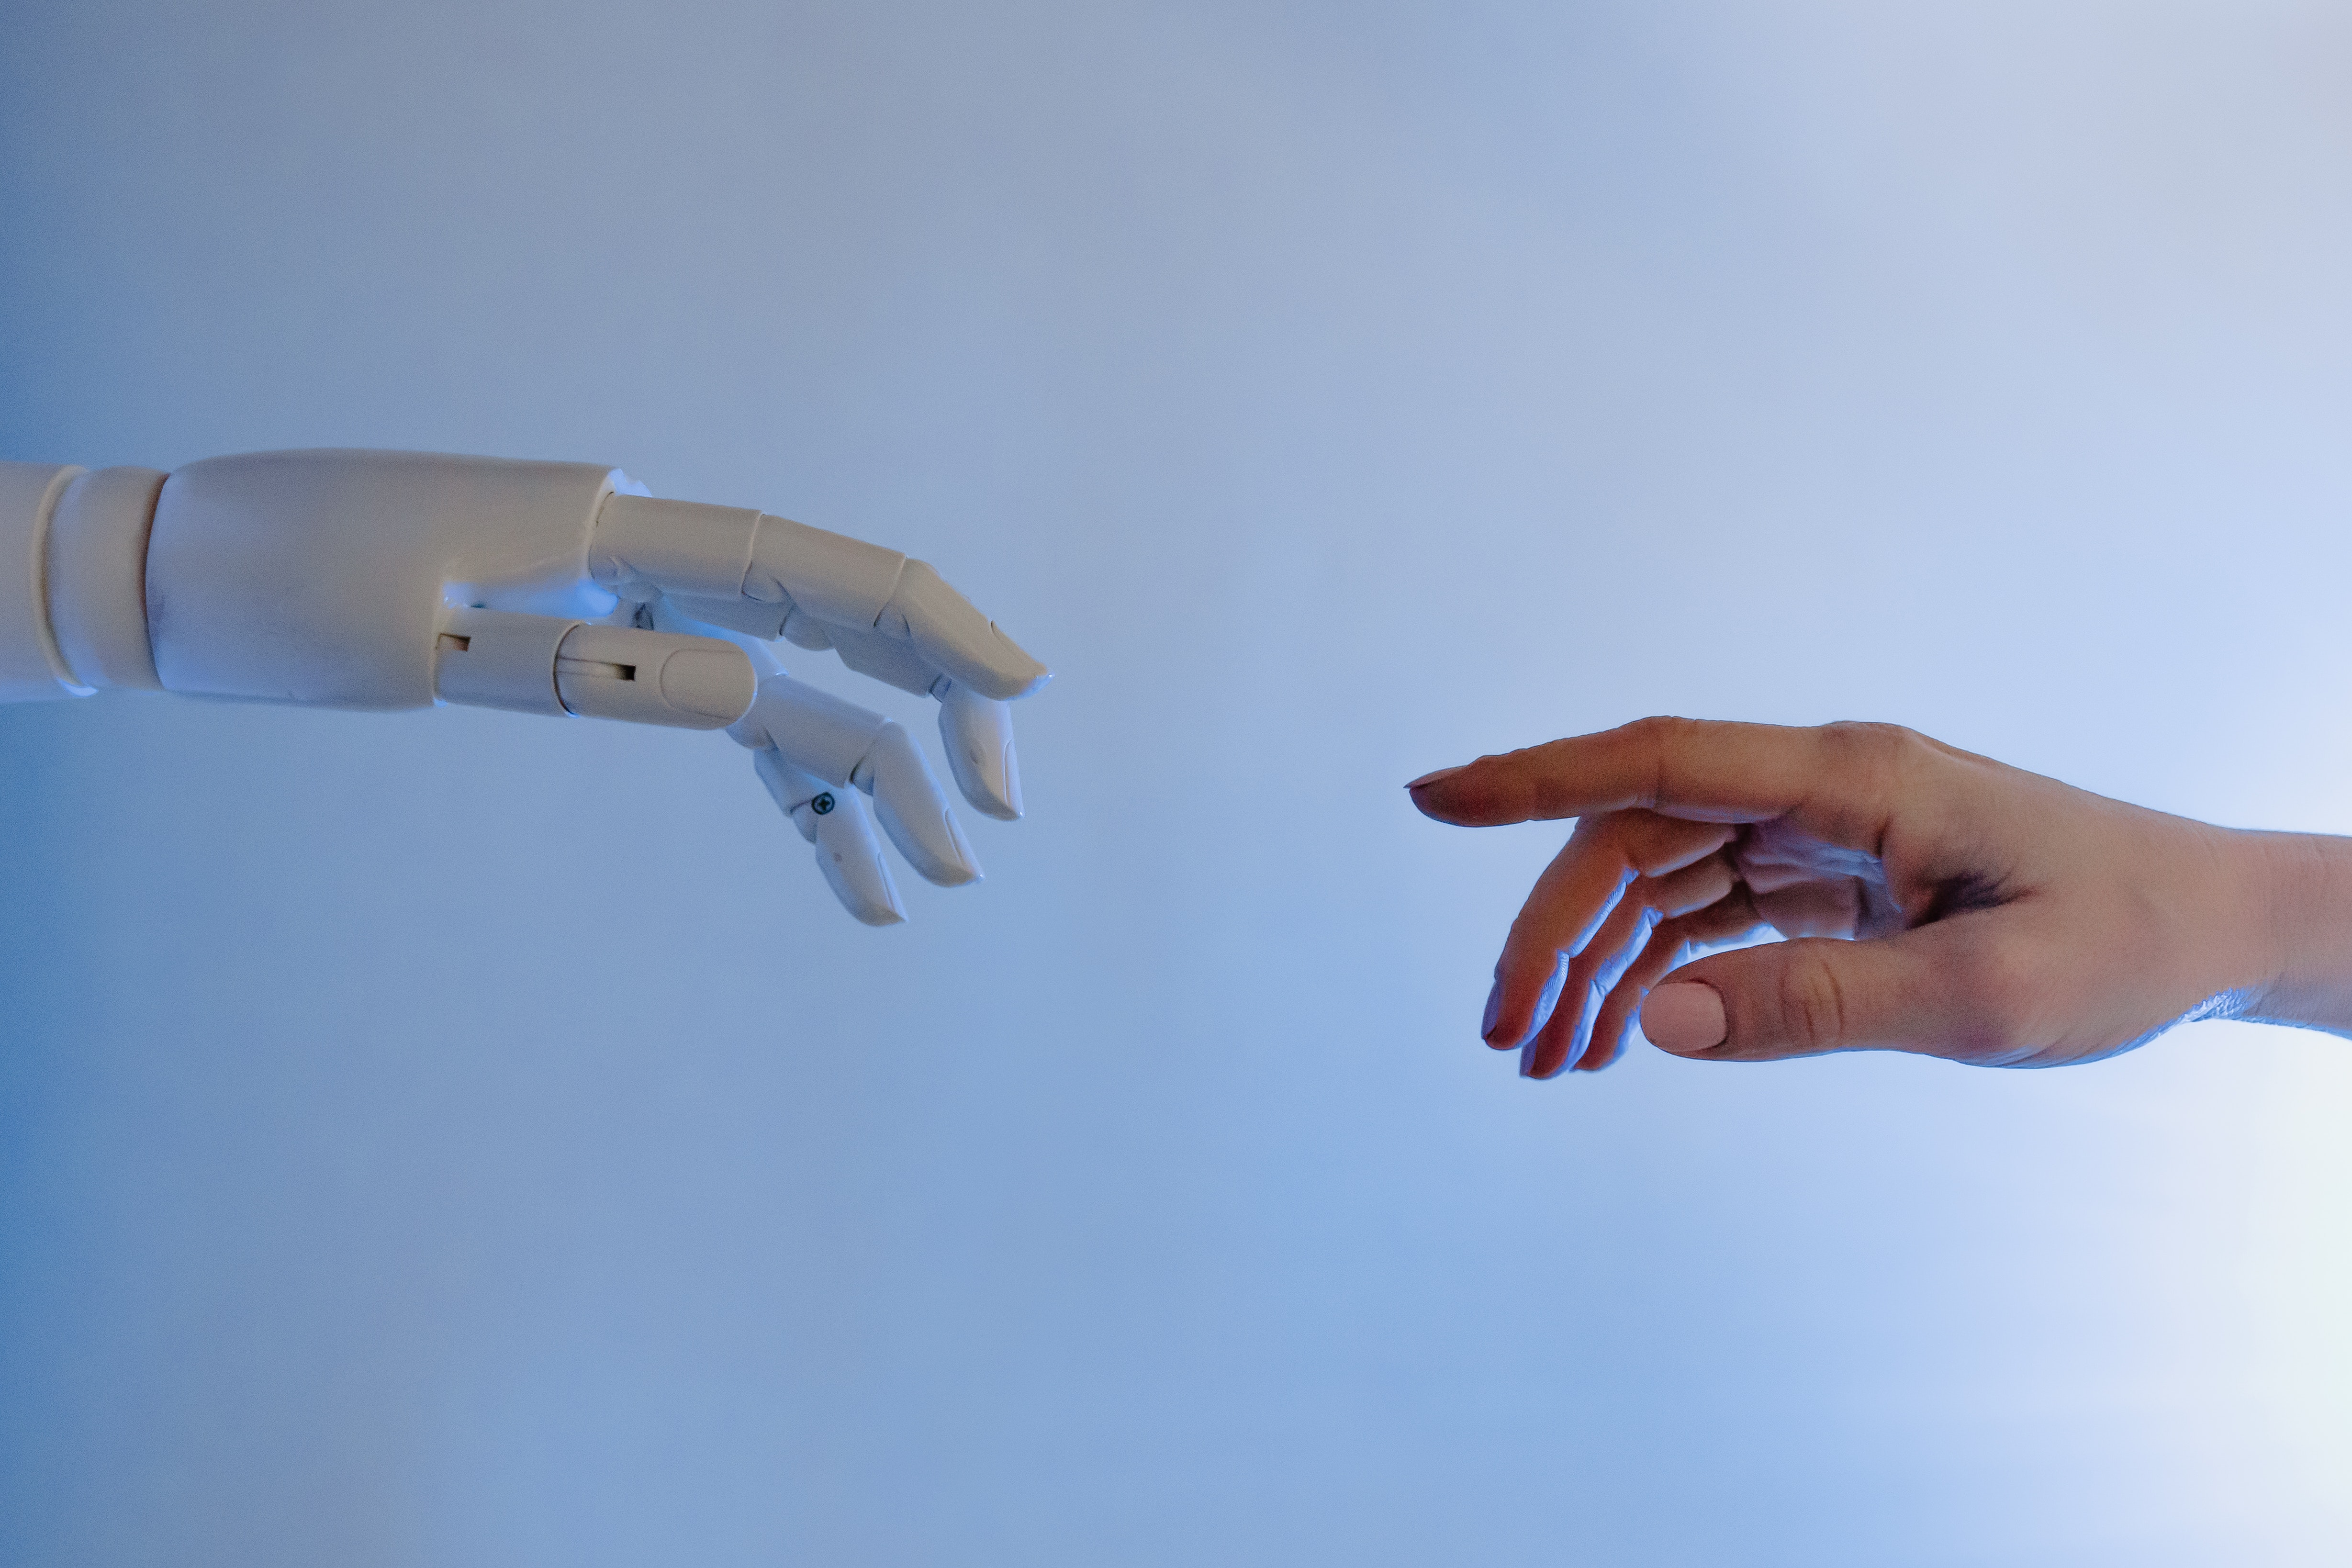
\includegraphics[width=10cm]{michelangelo_ki.jpg}
                     \centering
                 \end{figure}
                 \vspace{1cm}
                 {\Large Auszubildender Fachinformatiker Systemintegration \textbf{Hendrik Maier}\par}
                 \vfill
            \end{center}    
        \vspace*{\fill}
    \end{titlepage}
    
    %changing the layout after the titlepage
    %\newgeometry{top=1in,bottom=1in,right=0.5in,left=1.5in}
    \newgeometry{a4paper, left=3cm, right=5cm, top=2cm}

    \tableofcontents
    \newpage


% Begin of the Text
\chapter{Was ist eigentlich künstliche Intelligenz - Definition und Einleitung}

    %------------------------------------------------------------------------------------------------------------
    %MUSS NOCH NACHBEARBEITET WERDEN! WURDE NUR AUS DER ERSTEN VERSION KOPIERT
    %------------------------------------------------------------------------------------------------------------

    In den letzten Jahren hat der Begriff der \say{Künstlichen Intelligenz} (KI) als Schlagwort ein erhebliches Gewicht
    erlangt. Unterschiedlichste Quellen berichten von KI, als einer revolutionären Technologie, die die
    Art wie wir Leben von Grund auf verändert.
    Dabei beschränkt sich KI nicht nur auf ihr Herkunftsgebiete, die Informatik, sondern findet ihren Weg auch in
    Einsatzgebiete wie die Medizin und die Wirtschaft. Dort wird KI nicht nur zur Früherkennung
    von Krebs sondern auch zur Prognose von Aktienkursen genutzt. So unterschiedlich
    beide Anwendungsfälle auch klingen mögen, basieren beide auf der gleichen Technologie.\\

    Um eine Grundlage zu schaffen, möchte ich vorerst den Begriff der \say{Künstlichen Intelligenz}
    erläutern, um Klarheit um diesen oft genutzten und doch unklaren Begriff zu schaffen.
    Namensschöpfend war die 1956 abgehaltene \emph{Darthmouth Conference}\cite[57]{buchanan2005very}, 
    eine Versammlung auf der 
    Forschende erstmals zusammentrafen um die Möglichkeit von KI zu diskutieren.
    Der Begriff \emph{Intelligenz} kommt vom lateinischen \say{intelligere} was soviel wie
    einsehen, begreifen und erkennen bedeutet.\cite{piaget2000psychologie}
    \say{Künstlich} verweist in diesem Zusammenhang auf die unnatürliche Herkunft dieser Intelligenz.
    Da Erkenntnis und somit Intelligenz, immer etwas Geistiges ist\cite{duden2021erkenntnis}, könnnte
    man KI wie folgt definieren:
    \begin{displayquote}
        \say{Künstliche Intelligenz} beschreibt einen nicht-menschlichen
        unnatürlichen Geist, der die Fähigkeit besitzt, 
        durch das eigenständige Denken Erkenntnis zu erlangen.
    \end{displayquote}
    Dies, wenn man sich an der Bedeutung der Wort orientiert, ist eine Idealbeschreibung künstlicher Intelligenz.
    Da dies nicht dem aktuellen Forschungsstand entspricht, könnte man eine realere Definition schaffen mit der der unmittelbare
    Stand der Technologie passender abgebildet wird:
    \begin{displayquote}
        Eine \say{Künstliche Intelligenz} ist ein Computerprogramm, das 
        mit der Analyse von Statistiken Vorraussagen treffen oder Muster erkennen kann.
    \end{displayquote}
    Obwohl beide Definitionen sich augenscheinlich starkt unterscheiden, kann man die zweite Definition als Fundament für
    die erste Definition sehen. Um einen denkfähigen Geist zu erschaffen bedarf es Erfahrungen, die im Fall des Menschen
    das Gehirn lehren Situationen vorrauszusehen, bzw. Prognosen zu treffen und Zusammenhänge zu sehen.\footnote{Evolutionär
    gesehen ist der menschliche Geist und die 
    damit verbundenen Vorhersagen über die Realität
    das mächtigste Werkzeug im Kampf ums Überleben.}
    Computer haben keine Sinne, die sie mit der äußeren Welt verbinden und 
    müssen daher erst Statistiken, Daten oder Erfahrungen zugeführt kriegen.
    Dieses Zuführen muss im Moment noch der Mensch übernehmen.
    Einem Computer dadurch die eigenen Fähigkeiten zu lehren, macht wahrscheinlich ein Großteil der Faszination
    beim Entwickeln einer KI aus. Um dies zu bewerkstelligen ist Forschung in den unterschiedlichsten Feldern nötig,
    wozu nicht nur Informatik und Mathematik, sondern auch Psychologie, Linguistik und Philosophie\cite{buchanan2005very} gehören.\\

    Aus dieser Zusammenarbeit erwächst das Fachgebiet der \say{Künstlichen Intelligenz}, in welches
    im Folgenden Einblick gegeben werden soll.
    Durch die scheinbar universellen Anwendungsmöglichkeiten von KI, tut sich ein schier riesiges Gebiet an Teilthemen auf.
    Um die Zugänglichkeit zu gewährleisten, ist Ziel dieses Fachberichts nicht die komplette Durchleutung
    des Themas. Eher wird ein einführender Charakter angestrebt,
    der auf Geschichte, Funktionsweise und Philosophie von KI eingeht,
    um Anhaltspunkt zum ganzheitlichen Verstehen von KI zu geben.
    

\chapter{Der Traum vom mechanischen Helferlein - Geschichte}

    Wie auch bei vielen anderen neuzeitlichen Erfindungen, spielte Kultur in Form von Literatur eine entscheidende Rolle
    in der KI-Forschung. Erst durch die Vorstellungskraft von Autoren wie Isaac Asimov
    \footnote{bekannt durch: Die Foundation-Trilogie, derZweihunderjährige Mann}
    oder Jule Verne\footnote{bekannt durch: Zwanzig Tausend Meilen unter dem Meer, Die Reise zum Mittelpunkt der Erde}, 
    wurden Generationen von Forschenden inspiriert die Grenzen des Möglichen auszutesten. 
    Die Idee der KI ist dabei schon so alt wie unsere Zivilisation. 
    Schon der griechische Dichter Homer schrieb von mechanischen Dienern die den Göttern bei ihrem Mahl
    Wein nachschenkten\cite[53]{buchanan2005very}. Auch wenn diese Verwendung eines Robotors aus unserer heutigen
    industriellen Sicht eher banal erscheint, war ein solcher Apparat zu damaligen Zeiten visionär.
    Nicht weniger visionär, war die Vorstellung des Philosophen und Naturforschers Gottfried Wilhelm Leibniz der mechanische
    Richter imaginierte, die aufgrund von logischen Regeln Rechtsfälle zwischen Parteien aushandeln\cite[53]{buchanan2005very}.
    Vergleicht man diese Vorstellungen mit der heutigen Zeit, so sieht man das sich die Visionen der Menschen durch die Zeit hindurch
    nicht groß verändert haben. Beide Denker beschreiben dienende und logisch operiende Maschinen.
    Doch gestehen beide ihren erdachten Apparaten ein wesentliches Attribut nicht ein: Die Denkfähigkeit. 

    \section{Denkfähige Maschinen}
        Um dies zu wagen braucht es Mitte des 20. Jahrhunderts erst den britischen Mathematiker Alan Turing, 
        der mit seinem Gedankenexperiement, dem \say{Nachnahmungs - Spiel}, 
        die Frage nach intelligenten und denkenden Maschinen stellte.
        Dieses auch als \say{Turing-Test} bekannte Gedankenexperiment stellt seit dem einen 
        Richtwert für den Forschritt der KI-Forschung.\footnote{siehe Kapitel \say{Gedankenexperimente}, Abschnitt \say{The Imitation Game}}
        Diese neue Forschungsdisziplin entstand zur gleichen Zeit als Ergebnis 
        der Verbesserung der Halbleiter-Technologie, die als Basis für 
        moderne binäre Computersysteme gilt. Die dadurch vergrößerte Rechenkapazität und -leistung 
        eröffnete damals bisher nicht realisierbare Forschungsmöglichkeiten. 
        Seitdem finden KI-Forschende immer mehr Anwendungsmöglichkeiten um die Grenzen der KI immer weiter auszuweiten.
    
    \section{Menschen gegen Maschine}
        1997 erzeugt das Schreiben und Test von KI-Programmen, erstmals einen großes Medienecho, 
        als der von IBM programmierte Schachcomputer
        \say{Deep Blue} den damals amtierenden Schach-Weltmeister Gary Kasparov, schlug.\cite{chessbase2017kasparovdeepblue} 
        Die Komplexität von Schach war mit purer brutaler
        Rechnenleistung bisher noch nicht geknackt worden. Dazu bedarf es erst einem \say{Verständnis} von Schach dass bis zu diesem
        Zeitpunkt nur Menschen zugänglich war. Das Programm probierte also nicht mehr nur alle Züge aus, sondern prognostizierte die 
        Sinnvollsten. Damit wurde eine Zeitenwende eingeleitet und der breiten Öffentlichkeit die Macht von KI demonstriert.
        Das dadurch erschaffene Interesse beflügelte die KI-Forschung und weitete diese in mehr Anwendungsbereiche aus.
        In 2021 hatten ein Großteil der Menschen in ihrem Alltag schonmal Kontakt zu KI-Technologie. 
        Ob bei der Suche im Internet oder bei Nutzung einer Sprachsteuerung, steht im Hintergrund immer diese Technologie.
        Die Vorstellung von einem mechanischen Helferlein weicht allmälich dem Bild der universal anwendbaren künstlichen Intelligenz.
        

    \section{Zukunftsprognosen}
        Mit dem sich wandelnden Bild und mit den erweiterten technologischen Möglichkeit die den Entwicklern zur Verfügung stehen,
        stellt sich die Frage in welche Richtung sich KI entwickeln wird.
        Eine der bekanntesten Hypothesen, die diese Frage beantworten möchte, wurde 1993 vom US-Amerikanischen Mathematiker und 
        Informatiker Vernor Vinge aufgestellt und 2003
        erneut bestätigt. Vinge beschreibt ein spätestens 2030 auftretendes Ereignis, 
        welches er die \say{technologische Singularität}\cite[1]{vinge1993technological} nennt. 
        Er nennt mehrere Szenarien welche, direkt oder indirekt, 
        ein Entstehen einer denkfähigen superintelligenten Entität\footnote{Enität: Abstrakte Beschreibung eines existierenden/seienden Gegenstand, Objekts oder Wesens}
        beschreiben, die auf Computertechnologie basiert.
        Diese Enität soll die Intelligenz des Homo sapiens überschreiten\footnote{Menschen}
        und dadurch die Fähigkeit erlangen sich selbst zu verbessern.\\

        Betrachtet man Vinges Prognose für die nahe Zukunft
        und Homers Beschreibung von Wein ausschenkenden Dienern,
        wird ein möglicher Entwicklungsprozess sichtbar, dem jeglicher moderner Vergleich fehlt.
        Klar wird das eine solch selbstdenkende Form der KI, nicht nur Vorteile bringt. 
        Alleine die Programmierung der Ethik
        stellt Philosophen wie auch Programmierer
        vor ungelöste Probleme.\footnote{Wir haben keinerlei Vergleichwerte zu anderen Arten von Intelligenzen um zu
        beurteilen wie stark sich unsere Ethik im Vergleich unterscheidet.}
        Trotzdessen ist KI-Technologie die, mit am stärksten antizipierte Technologie des 21. Jahrhunderts,
        wessen Geschichte noch lange nicht beendet ist.




\chapter{Schwache versus starke Arten von KI}
    Vinges Zukunftsprognose\cite[1]{vinge1993technological} beschreibt eine Art KI die,
    im Vergleich zu Leibniz und Homers Überlegungen unterschiedlicher nicht sein könnte.
    Um zu konkretisieren was genau diese beiden Arten von KI unterscheidet, nehme ich
    mir Isaac Asimovs Roman \say{Der Zweihundertjährige Mann} zur Hilfe.
    Darin beschreibt Asimov einen Roboter, der sowohl als mechanischer Diener, als
    auch als selbstdenkender kreativer Künstler agiert.\cite{asimov2000der}
    Unwissend macht Asimov somit eine Einteilung in zwei Arten von KI,
    die hilft den Entwicklungsfortschritt zu projizieren.
    Die Rede ist von der schwachen KI, dem logisch agierenden Diener, und
    starker KI, dem kreativen Künstler.

    \section{Schwache KI}
        Als \say{schwache künstliche Intelligenz} bezeichnet man aktuell jedes,
        mit maschinellem Lernen trainierte Computerprogramm. 
        Dazu gehört Spracherkennungssoftware, wie zum Beispiel Alexa oder Siri,
        sowie Gesichtserkennung als auch jegliche Forschungs- oder Militärsoftware, die KI-Technologie benutzt.
        Alle diese Anwendungsbeispiele benötigen den Menschen als ausführenden und lehrenden (bzw. trainierenden)
        Bezugspunkt.
        Ohne den Menschen oder ein vom Menschen vorbereiteten Mechanismus, ist es zum derweiligen Zeitpunkt
        keinem Computerprogramm oder keiner Maschine möglich, aus eigener Initiative zu handeln.
        Genau diese fehlende Initiative ist das charakterisierende Attribut einer \say{schwachen KI}.
        Falls eine KI jedoch Initiative zeigen und eigene Intentionen verfolgen würde, würde dies 
        ihre Denkfähigkeit bestätigen und somit eine neue Entwicklungsstufe erreicht werden.
    \newpage

    \section{Starke KI}
        Die nächste Entwicklungstufe künstlicher Intelligenz ist
        die \say{starke künstliche Intelligenz}.
        In der Theorie hat starke KI jede Fähigkeit die schwache KI ebenfalls hat.
        Sie wird daher als erweiterte Form angesehen und nicht als unterschiedliche
        Technologie bewertet.
        Die Erweiterung besteht in der Fähigkeit zum selbst- oder eigenständigen Denken. Obwohl
        starke KI indirekt den Menschen als initialisierendes Glied benötigt,
        kann sie Aufgaben autark und ohne direkte Anweisungen erledigen.
        Um das voranschreiten künstlicher Intelligenz zu Erkennen, kann
        man das betreffende Computerprogramm dem \say{Turing-Test}
        \footnote{siehe Kapitel \say{Gedankenexperimente}, Abschnitt \say{The Imitation Game}} unterziehen,
        welcher die Denkfähigkeit einer Maschine mit der eines Menschen vergleicht.
        Strittig ist, ob eine Computerprogramm jemals so Denken kann wie ein 
        Mensch.\footnote{siehe Kapitel \say{Gedankenexperimente}, Abschnitt \say{Das Chinesische Zimmer}}
        Eine solche starke KI, dessen Denkfähigkeit sich mit der eines Menschen vergleichen lässt, wird
        von Forschenden oft als \say{Superintelligenz} bezeichnet, da aus dem Erreichen einer solchen Intelligenzstufe
        eine selbstständige Verbesserung der eigenen Fähigkeit gefolgert wird.
        Ähnlich zu Vernor Vinges Vorstellungen, beschreibt der, an der Universität von Oxford lehrende Professor
        Nick Bostrom, den Begriff der \say{Superintelligenz} wie folgt:
        \begin{displayquote}
            \say{Mit einer \say{Superintelligenz} meinen wir einen Intellekt
            der, in jedem denkbaren Feld, viel schlauer als irgendein menschliches Gehirn ist.
            Dazu zählen wissenschaftliche Kreativität, allgemeine Weisheit und jegliche soziale Fähigkeiten.}\cite{superintelligence1998bostrom}
        \end{displayquote}
        Zwar legen sich Vinge sowohl als auch Bostrom nicht auf eine starke KI als Übergangspunkt
        zur \say{Technologischen Singularität}\cite{vinge1993technological} oder \say{Superintelligenz}\cite{superintelligence1998bostrom} fest,
        jedoch beziehen mehrere ihrer Szenarien die KI-Technologie mit ein.
        Um ein Stufe von Autarkie zu erreichen, die eine starke KI gewährt, muss eine neue Methode
        des Wissensgenerierung in die KI-Technologie implementiert werden, die selbstständiges Erarbeiten von Wissen begünstigt.
        




\chapter{Technische Grundlagen}
     Wie schon zuvor beschrieben ist eine KI nichts anderes als ein Computerprogramm,
     welches durch die Analyse von Statistiken oder Datenpunkten, Prognosen abgeben oder Muster erkennen kann.
     Diesen Prozess der Analyse nennt man maschinelles Lernen (ML).
     In diesem Prozess spielen das Feld der Erkenntnistheorie, Mathematik und Informatik 
     maßgebende Rollen. Jede Disziplin erfüllt dabei eine eigene Aufgabe.
     Um eine Analyse durchzuführen benötigt es einen methodischen Ansatz.
     Die Erkenntnistheorie stellt hierfür die Methoden zur Verfügung.\footnote{Diese werden auch von 
     Menschen bewusst oder unbewusst beim Lernen und Verstehen verwendet.}
     Die Mathematik gibt die Möglichkeit diese Methoden in eine allgemeine anwendbare Sprache zu übersetzen.
     Die praktische Anwendung geschieht durch die Informatik in Form von Programmierung.
     Durch die Zusammenarbeit von diesen verschiedenen Disziplinen ist es
     möglich mithilfe von ML ein Modell (ML-Modell) durch Training zu generieren,
     welches zukünftige Problemstellungen mit anhand gelernten (trainierter) Daten lösen kann.
        
    \section{Wie betreibt man maschinelles Lernen?}
        Im Vorfeld des Lernes, ist es wichtig den Sinn der KI zu bestimmen.
        Denn je nach Anwendungsfeld oder Ziel der KI, kommt eine andere Methode und somit
        ein anderer Algorithmus zum Einsatz. Jede Methode bietet verschiedene Algorithmen,
        die jeweils eigene Vorgehen verfolgen. Unter den Algorithmen kann man
        dann den passenden auswählen, der die Zielvorgabe erfüllt.

    \newpage    

    \subsection{Top-Down Methode (Deduktiv)}
        Die erste Methode die beim ML angewandt wird, bezeichnet man als Top-Down Methode,
        welche deduktiver Natur ist. Dies bedeutet das man mithilfe  allgemein anerkannter Regeln
        auf spezielle Fälle schließt.\cite{dundi2021unileipzig} 
        \footnote{Beispielweise weiß ich, dass die Sonne warm ist. Da draußen die Sonne scheint, schließe ich daraus,
        dass es draußen warm sein muss. Das bedeutet aber nicht das Deduktion der sicherste Weg des 
        Schlussfolgern ist. Draußen kann die Sonne scheinen und es kann kalt sein weil Winter ist.}\\

        Im Kontext des ML bedeutet das, dass immer vorgefertigte Regeln, Features und Targets, vorhanden sein müssen.
        Diese Regeln werden im Normalfall vom Menschen, in der Form von Traingsdaten, definiert. Daher spricht man bei dieser Methode
        auch vom beaufsichtigten Lernen bzw. dem Supervised Learning.

        \subsubsection{Supervised Learning}
            Mit dieser Art des Lernens ist es möglich zwei verschiedene 
            Problemkategorien zu lösen\cite{supervisedlearning2021ibm}:

            \begin{itemize}
                \item{Klassifikationsprobleme}
                \item{Regressionsprobleme}
            \end{itemize}

            Diese können durch jeweils eigene Algorithmen bearbeitet werden.
            Als Klassifikationsprobleme bezeichnet man Situationen in den ein bestimmter Wert zu einer
            bestimmten Auswahl von Gruppen zugeordnet werden soll. Das bedeutet, dass es eine Zielvariable gibt, die
            nur eine vordefinierte Anzahl von Werten annehmen kann.\cite{kibuisness2021supervised}
            Der Algorithmus versucht also die Daten aufzuteilen.
            Möchte man eine bestimmte Prognose aufgrund von vorherigen Werten erhalten,
            handelt es sich um Regressionsproblem.\cite{kibuisness2021supervised}
            Dabei versucht der Algorithmus einen Trend zu Erkennen um den zukünftigen Zustand der Zielvariable zu ermitteln. 
            Das Lösen beider Problemarten hängt dabei vom Vorherigen Kennzeichnen bzw. Labeln der Datenpunkte ab.
            Nur mit einer logisch differenzierbaren Einteilung in Features und jeweilig ein Target, 
            kann ein Algorithmus das angegebene Problem lösen.
            Ein Target ist eine Zielvariable die ermittelt wird. 
            Ein Feature steht als Anhaltspunkt zu Verfügung.
            Ein bestimmtes Target
            besitzt also eine bestimmte Anzahl an Features, durch welches es charakterisiert wird.
            Bei der Analyse der Zusammengehörigkeit von Features eines Targets, wird nun ein Modell
            generiert, mit dem eine Prognose gemacht oder die Zugehörigkeit zu einer Gruppe bestimmmt werden kann.
            Vorteil dieser Art des Lernens ist, ein hoher Einfluss auf das Ergebnis des Lernprozesses,
            da man die Möglichkeit hat eigene Features und Targets sehr spezifisch zu definieren.
            Nachteil des Supervised Learning ist die im Vergleich lange Trainingszeit eines Modell
            und eine hohe Fehlerquote durch schlechtes Kennzeichnen der Trainigsdaten, durch den Menschen.
            
           
%        \subsection{Pre-Labeled (Test-und Training-) Data}
%        \subsection{Specific Application Area}
%        \subsection{Pro \& Contra}
        
    \subsection{Bottom-Up (Induktiv)}
        Die zweite Methode die beim ML angewandt wird betrachtet Daten ohne davor irgendeine Form von Regeln zu beachten.  
        Die Daten werden unvoreingenommen und ohne jede Grundlage betrachtet.
        Aufgrund von logischen Zusammenhängen werden dann Regeln abgeleitet womit sich die Daten erklären lassen können.
        Diese Method wird, bildgebend, als Bottom-Up oder auch als induktiv\cite{dundi2021unileipzig} bezeichnet.
        
        \footnote{Beispielweise beobachte ich, dass jeden morgen die Tram zu gleichen Uhrzeit kommt. Daraus schließe ich 
        dass sie nach einem Fahrplan verkehrt.}

        Da diese Methode keine Grundlagen benötigt, spricht man
        im Kontext des ML vom unbeaufsichtigtem Lernen bzw. vom Unsupervised Learning.
        \subsubsection{Unsupervised Learning}
            Beim Unsupervised Learning gibt es drei Lösungsansätze\cite{unsupervisedlearning2021ibm}:
            \begin{itemize}
                \item{Clustering}
                \item{Assoziation}
                \item{Dimensionsreduzierung}
            \end{itemize}
            Wie auch beim Supervised Learning gibt es auch zu diesen Ansätzen, verschiedene
            Algorithmen, die jeweils eigene Lösungswege verfolgen.
            Der hauptsächliche Unterschied der zum Supervised Learning besteht, ist das Eingreifen
            des Menschens bei der Vorbereitung der Datenpunkte. Unsupervised Learning Algoritmen
            benötigen keinerlei Anhaltspunkte, sondern betrachten unvoreingenommen  nur die rohen Daten.
            Beim Clustering, was soviel wie \say{Zusammenhäufen} bedeutet, wird dies am besten repräsentiert.
            Dabei werden nur auf Grund von Gemeinsamkeiten und Unterschieden der Datenpunkte, Gruppen gebildet.\cite{clustering2021elementai}
            Dies ist nützlich wenn man große Mengen an Daten hat, über die man Einsicht gewinnen möchte.
            Möchte man hingegen die Zusammenhänge von Daten verstehen, 
            bieten sich Assoziations-Algorithmen an.\cite{apriori2019sciencedata}
            Ein typisches Anwendungsgebiet von Assoziations-Algorithmen ist die Analyse des Kaufverhaltens eines Kunden.
            Dabei repräsentiert ein gekaufter Artikel einen Datenpunkt. 
            In vergangenen Einkäufen erworbene Artikel werden nun 
            in ihrem Bezug zueinander analysiert und eine Wahrscheinlichkeit ausgerechnet, mit der sich
            das Kaufen oder Nicht-Kaufen vorhersagen lassen kann. Die Dimensionsreduzierung kann
            ähnliche Ergebnisse ausgeben, in dem sie wichtige und unwichtige Datenpunkte trennen kann.
            Diese Art des Unsupervised Learning wird hauptsächliche bei der Vorbearbeitung von Datensets eingesetzt,
            die im späteren Gebrauch beim Supervised Learning benutzt werden.\cite{unsupervisedlearning2021ibm}
            Unrelevante Features werden von den Relevanten getrennt, wodurch die Berechnungszeit und die Übersicht
            verbessert wird.
            
    \subsection{Semi-Supervised Learning}
        Wie der Einsatz von Dimensionsreduzierung zeigt, sind die Grenzen zwischen Supervised und Unsupervised Learning fließend.
        Ein konkreter Fall bei den beide Seiten zusammenarbeiten ist das Semi-Supervised Learning.
        Dabei wird ein kleiner Teil von gekennzeichneten Daten und ein größerer Teil von ungekennzeichneten Daten verwendet,
        um ein ML-Modell zu generieren.\cite{semisupervised2021mlmastery}


%        \subsection{Unlabeled Training Data (no Test, no Accuary)}
%        \subsection{Wide Range of Output}
%        \subsection{Pro \& Contra}
            
%    \section{deep learning - neuronale netzwerke}
%        \subsection{kann induktiv oder deduktiv arbeiten!}
%        \subsection{wie funktionieren neuronale netzwerke?}
%        \subsection{implementierung eines menschlichen gehirn mithilfe von unsupervised learning}

\chapter{Gedankenexperimente}
    Um neue Forschungsgebiete zu erschließen, ohne dabei handfeste Ansätze zu haben,
    bieten sich Gedankenexperimente als nützliche Hilfsmittel an.
    Mit deren Hilfe lassen sich unreale Situationen konstruieren, durch welche man logische Schlussfolgerungen ziehen kann.
    Im Folgenden werden zwei Gedankenexperimente beschrieben, die trotz ihres betrachlichen Alters, in der KI-Forschung
    immer noch Relevanz besitzen. Beide zeichnen sich dadurch aus, dass sie dem Denkenden die Möglichkeit geben sich in die
    Rolle einer Maschine zu versetzten. Dadurch kann der Denkende die Kernfrage der KI-Forschung aus einer anderen
    bzw. aus einer eigenen Perspektive erleben. 

    \section{The Imitation Game - Das Nachahmungs-Spiel}
        Mitte des 20. Jahrhunderts stellte der britische Mathematiker Alan Turing als einer der ersten
        die Frage, ob es möglich sei, dass Maschinen denken können. Dies gilt seitdem als hauptsächliche
        Kernfrage der KI-Forschung. Um diese Frage zu beantworten schlägt Turing das \say{Imitation Game} oder
        auch \say{Nachahmungs-Spiel}, als Test für die Denkfähigkeit von Maschinen vor. Als Maschine schlägt er
        explizit einen digitalen oder elektronischen Computer vor und schließt biologische Möglichkeiten,
        wie einen aus einer Zelle gezüchteten Menschen komplett aus.\cite[435]{turing1950computing}
        Eine vollständige Abkapselung einer digitalen Maschine, als eigenständiges Gerät ist jedoch nicht möglich, da sie auf dem
        Fundament von menschlichen Prinzipien konstruiert worden ist. Maschinen müssen immer als menschgemacht betrachtet werden.
        Mit diesem Hintergrundwissen schlägt er folgendes Spiel vor:
        \begin{displayquote}
            Für das Nachahmungs-Spiel werden insgesamt drei Spieler*innen benötigt. Ein Mann (A), eine Frau (B) und ein*e
            Fragesteller*in (C). Die Aufgabe des/der Fragesteller*in ist herrauszufinden wer von beiden die Frau ist.
            Dabei sitzt er/sie in einem anderen Raum als die beiden. Der/Die Fragesteller*in kennt beide Parteien
            nur unter X und Y, womit er am Ende des Spiel jeweils A und B identifiziert. Ziel von A ist es den/die Fragesteller*in
            fehlzuleiten. B verfolgt das Ziel, den/die Fragesteller*in zur richtigen Antwort zu leiten.
            \cite[433]{turing1950computing}
        \end{displayquote}
        In diesem Gedankenexperiement wird der Mann (A) nun durch eine Maschine ersetzt, die seine Aufgabe übernimmt und
        sich als Frau (B) ausgeben soll. Der Austausch von Informationen erfolgt dabei über Maschinenschrift, damit
        der/die Fragesteller*in keine Schlussfolgerungen über Stimme oder Schrift ziehen kann.\cite[433]{turing1950computing}
        Bei diesem Test geht es nicht darum akutelle Maschinen zu betrachten und einen entgültigen Schluss zu ziehen, es geht
        eher darum, sich eine Maschine vorzustellen die diesen Test bestehen kann. Damit eine Maschine diesen Test erfolgreich abschließt,
        muss sie das Spiel mit einer 70\%iger Genauigkeit gewinnen.\cite[1]{oppy&dowe2020turingtest}
        

    \section{Das Chinesische Zimmer}
    Das Chinesische Zimmer ist ein Gedankenexperiment vom Philosophen John Searle, welches
    versucht, die Frage nach der erfolgreiche Entwicklung einer starken Künstlichen Intelligenz zu verneinen.
    Searles These ist, dass kein Computer jemals wie ein Menschen denken kann,
    obwohl sowohl der Computer als auch das Gehirn Systeme sind, die Symbole verarbeiten.\cite{nimtz2013chinesische}
    Dies begründet er mit folgendem Gedankenexperiment:
    \begin{displayquote}
        \say{Stellt euch vor ich wäre in einem geschlossenen Raum mit einem großen Haufen chinesischer Texte.
        Ich kann weder Chinesisch sprechen noch lesen oder schreiben.
        Ebenfalls könnte ich chinesische von keiner anderen, wie beispielweise russischer, japanischer Schrift unterscheiden.
        Chinesische Schriftzeichen haben keine erkennbare Bedeutung und sind nur Formen für mich.\\

        Nun stellt euch vor ich würde einen zweiten Stapel erhalten. Dieser Stapel enthält weitere
        Chinesische Schriftzeichen sowie englische formale Regeln, die ich ohne Probleme verstehe.
        Diese formalen Regeln geben mir die Möglichkeit die chinesischen Schriftzeichen
        anhand ihrer Form zu identifizieren.\\

        Nun kriege ich einen dritten Stapel mit weiteren chinesischen Schriftzeichen und englisch 
        Anweisungen die mir sagen wie ich
        diese neuen chinesischen Zeichen mit den Vorherigen vergleiche um bestimmte chinesische Zeichen zurückzugeben.\\

        Mit der Zeit werden die Leute außerhalb des Raumes immer besser, mir englische Anweisungen zu schreiben und
        ich werde immer besser diese auch zu verstehen, so dass meine Antworten ununterscheidbar von denen eines
        gebürtigen Chinesen werden. Doch verstehe ich, was ich an Chinesisch von mir gebe?}
        \cite[1]{searle1999chinese}
    \end{displayquote}
    Searle versucht mit diesem Gedankenexperiment den Unterschied zwischen
    Syntaktik\footnote{Syntaktik (Syntax): Wie stellt man Zeichenketten zusammen, sodass sie Sinn ergeben?}
    und Semantik\footnote{Semantik: Was genau ist die Bedeutung hinter einem Wort?}
    greifbar zu machen.
    Ein Computer der keinerlei Verbindung in die Realität eines Menschen hat, kann zwar Regel lernen, die ihm die
    Welt der Menschen näher bringt, jedoch kann er niemals voll und ganz \emph{verstehen} oder auch \emph{begreifen},
    wie ein Mensch denkt. Damit setzt Searle eine eher negative Prognose auf den Forschritt, den die KI-Forschung
    machen oder besser gesagt, nicht machen wird.


%\chapter{Schlussfolgerung}
%    \section{Unterschied Mensch und Maschine}
%        Im vorherigen wurde der Begriff, die Arten sowie die Technologie an sich beschrieben und erläutert.
%        Doch um wahrhaftiges Verständnis von künstlicher Intelligenz zu gewinnen, braucht es einen
%        Vergleich der viel näher an dem eigenen Verständnis von Intelligenz liegt.
%        Die Rede ist vom direkten Vergleich mit dem Menschen.
%
%    \section{Menschen lernen sich selbst besser kennen wenn sie KI erforschen}
%            
%    \section{Was Maschinen vom Menschen unterscheidet}

\chapter{Fazit/Schlussfolgerung}
    Trotz ihres jungen Alters ist \say{Künstliche Intelligenz} eine heute schon verbreitet eingesetzte Technologie.
    Durch die Zusammengreifen verschiedenster Forschungsdisziplinen ist es den Menschen gelungen
    Maschinen zu konstruieren, die ihre eigenen Fähigkeiten imitieren und sogar effizienter ausführen können.
    Dies tun sie in dem sie Daten mit bestimmten Algorithmen analysieren, wodurch sie Muster erkennen und Prognosen voraussagen können.
    Damit wird ein Menschheitstraum wahr der schon seit Beginn unserer Zivilisation Denker und Visionäre beschäftigt.
    Ob Maschine nicht nur effizient sondern auch kreativ arbeiten können ist strittig.
    Dieser Unterschied zwischen einer \emph{logisch} oder \emph{kreativ} denkenden Maschine,
    führt uns im Kontext der aktuellen KI-Forschung an die Schwelle eines Zeitenwandels.
    Der Begriff der KI verbindet sich immer weiter mit dem Begriff der Superintelligenz.
    Um aus einer Maschine ein bewusstes Wesen zu machen sind neue Methoden der Wissengewinnung nötig.
    Bisherige KIs arbeiteten überwiegend mit der Top-Down-Methode bei der Regeln vorgegeben sind.
    Neuere unabhängigere KIs arbeiten hingegen mit der Bottom-Up-Methode, die eine Problemstellung 
    ohne vorgegebene Regeln bearbeiten können.
    Hier wird sichtbar dass die Bottom-Up-Methode die vielversprechenste Methode des Lernes, für zukünftige selbstdenkende Formen
    der KI sein wird.
    Eine solche Form der KI birgt viel Vorteile und Risiken.
    
    
    
     



    \printbibliography[title={Quellenverzeichnis}]

\end{document}
